\documentclass[aspectratio=169]{beamer}
%\documentclass{beamer}
\beamertemplatenavigationsymbolsempty
\usecolortheme{beaver}
\setbeamertemplate{blocks}[rounded=true, shadow=true]
\setbeamertemplate{footline}[page number]
%
\usepackage{tikz}
\setbeamertemplate{itemize item}{%
    \tikz{\fill[blue] (0,0) -- (-0.2,0.1) -- (-0.2,-0.1) -- cycle;}%
}

\usepackage[utf8]{inputenc}
\usepackage{bm}
\usepackage[english,russian]{babel}
\usepackage{amssymb,amsfonts,amsmath,mathtext}
\usepackage{subfig}
\usepackage[all]{xy} % xy package for diagrams
\usepackage{array}
\usepackage{bm}
\usepackage{multicol}% many columns in slide
\usepackage{hyperref}% urls
\usepackage{hhline}%tables
\usepackage{mathtools}
\usepackage{graphicx}
\captionsetup[subfigure]{font={small},labelfont={small}}
\usepackage{adjustbox}
% Your figures are here:
\graphicspath{ {fig/} {../fig/} }
\newtheorem{theorem_rus}{Теорема}
\newtheorem{lemma_rus}{Лемма}
\setbeamertemplate{theorems}[numbered]
\setbeamertemplate{caption}[numbered]
\usepackage{ragged2e}
\usepackage[T1]{fontenc} % Кодировка шрифтов для западных языков
\usepackage[utf8]{inputenc} % Кодировка UTF-8
\usepackage[english]{babel} % Поддержка английского языка

\usepackage[style=authoryear,language=english]{biblatex}
\addbibresource{references.bib} % Файл с библиографией
\justifying
% latin bold lower
\newcommand{\ba}{\mathbf{a}} 
\newcommand{\bc}{\mathbf{c}} 
\newcommand{\be}{\mathbf{e}} 
\newcommand{\bh}{\mathbf{h}} 
\newcommand{\bp}{\mathbf{p}} 
\newcommand{\bt}{\mathbf{t}} 
\newcommand{\bs}{\mathbf{s}} 
\newcommand{\bu}{\mathbf{u}} 
\newcommand{\bv}{\mathbf{v}} 
\newcommand{\bw}{\mathbf{w}} 
\newcommand{\bx}{\mathbf{x}} 
\newcommand{\by}{\mathbf{y}} 
\newcommand{\bz}{\mathbf{z}} 

% latin bold upper
\newcommand{\bA}{\mathbf{A}} 
\newcommand{\bB}{\mathbf{B}} 
\newcommand{\bC}{\mathbf{C}} 
\newcommand{\bI}{\mathbf{I}} 
\newcommand{\bJ}{\mathbf{J}} 
\newcommand{\bL}{\mathbf{L}} 
\newcommand{\bM}{\mathbf{M}} 
\newcommand{\bP}{\mathbf{P}}
\newcommand{\bQ}{\mathbf{Q}} 
\newcommand{\bR}{\mathbf{R}} 
\newcommand{\bT}{\mathbf{T}} 
\newcommand{\bU}{\mathbf{U}} 
\newcommand{\bV}{\mathbf{V}} 
\newcommand{\bW}{\mathbf{W}} 
\newcommand{\bX}{\mathbf{X}} 
\newcommand{\bY}{\mathbf{Y}} 
\newcommand{\bZ}{\mathbf{Z}} 

% latin cal upper
\newcommand{\cF}{\mathcal{F}} 
\newcommand{\cG}{\mathcal{G}} 
\newcommand{\cI}{\mathcal{I}} 
\newcommand{\cL}{\mathcal{L}} 
\newcommand{\cM}{\mathcal{M}} 
\newcommand{\cN}{\mathcal{N}} 
\newcommand{\cS}{\mathcal{S}} 
\newcommand{\cT}{\mathcal{T}} 
\newcommand{\cW}{\mathcal{W}} 
\newcommand{\cX}{\mathcal{X}} 
\newcommand{\cZ}{\mathcal{Z}} 

% latin bb upper
\newcommand{\bbE}{\mathbb{E}} 
\newcommand{\bbI}{\mathbb{I}} 
\newcommand{\bbP}{\mathbb{P}} 
\newcommand{\bbR}{\mathbb{R}}
\newcommand{\bbX}{\mathbb{X}} 
\newcommand{\bbY}{\mathbb{Y}}
\newcommand{\bbW}{\mathbb{W}} 

% greek bold lower
\newcommand{\bepsilon}{\boldsymbol{\epsilon}} 
\newcommand{\btheta}{\boldsymbol{\theta}} 
\newcommand{\blambda}{\boldsymbol{\lambda}} 
\newcommand{\bpi}{\boldsymbol{\pi}} 
\newcommand{\bmu}{\boldsymbol{\mu}} 
\newcommand{\bsigma}{\boldsymbol{\sigma}} 
\newcommand{\bphi}{\boldsymbol{\phi}} 

% greek bold upper
\newcommand{\bSigma}{\boldsymbol{\Sigma}} 

\DeclareMathOperator*{\argmin}{arg\,min}
\DeclareMathOperator*{\argmax}{arg\,max}

% transpose
\newcommand{\T}{^{\text{\tiny\sffamily\upshape\mdseries T}}}


\newcommand{\bb}{\mathbf{b}}
\newcommand{\bq}{\mathbf{q}}
\newcommand{\bS}{\mathbf{S}}
\newcommand{\bH}{\mathbf{H}}

\newcommand{\bE}{\mathbf{E}}
\newcommand{\bF}{\mathbf{F}}
\newcommand{\bomega}{\boldsymbol{\omega}}

\newcommand{\bgamma}{\boldsymbol{\gamma}}
\newcommand{\bdelta}{\boldsymbol{\delta}}
\newcommand{\bPsi}{\boldsymbol{\Psi}}
\newcommand{\bpsi}{\boldsymbol{\psi}}
\newcommand{\bxi}{\boldsymbol{\xi}}
\newcommand{\bchi}{\boldsymbol{\chi}}
\newcommand{\bzeta}{\boldsymbol{\zeta}}
\newcommand{\beps}{\boldsymbol{\varepsilon}}
\newcommand{\bZeta}{\boldsymbol{Z}}
% mathcal

\newcommand{\cY}{\mathcal{Y}}
\newcommand{\dH}{\mathds{H}}
\newcommand{\dR}{\mathds{R}}
%----------------------------------------------------------------------------------------------------------
\title[\hbox to 56mm{Краткое название}]{Robust Detection of AI-Generated Images}
\author[Г.\,В.~Килинкаров]{Георгий Валерьевич Килинкаров\\
\small Научный руководитель: к.ф.-м.н. А.\,В.~Грабовой \\
\small Ассистент: Д.\,Д.~Дорин}
\institute{Анализ данных ФПМИ МФТИ}
\date{2025}

%----------------------------------------------------------------------------------------------------------
\begin{document}
%----------------------------------------------------------------------------------------------------------
\begin{frame}
\thispagestyle{empty}
\maketitle
\end{frame}

%----------------------------------------------------------------------------------------------------------
\begin{frame}{Цель и постановка задачи}
\begin{block}{Цель работы}
    Построить модель классификации изображений на машинно-сгенерированные и оригиальные, устойчивую к методам генерации. 
\end{block}
\begin{block}{Постановка задачи}
Задана выборка $$\mathfrak{D} = \{\bm{x_i}, y_i \},\ i= 1, ..., N,$$ где $\bm{x_i} \in \mathbb{N}_0^{H \times W \times C}$~--- изображение размера $H \times W \times C$, $y_i \in \{ 0, 1\}.$ \\

Необходимо построить отображение $\bm{F}: \mathbb{N}_0^{H \times W \times C} \rightarrow \{ 0, 1 \}.$

Для нахождения оптимального отображения \( \bm{F}^* \) в классе моделей \( \mathcal{F} \) используется Binary Cross-Entropy Loss (BCE):
\[
	\bm{F}^* = \arg\min_{\bm{F}^* \in \mathcal{F}} \operatorname{BCE}(F).
\]
\end{block}
\end{frame}
%----------------------------------------------------------------------------------------------------------
\begin{frame}{Artifact}
В работе рассматривается датасет данных Artifact. Датасет включается в себя реальные изображения и 25 методов генерации изображений, включая 13 GANs, 7 диффузионных, и 5 других методов генерации. 
\begin{figure}
\centering
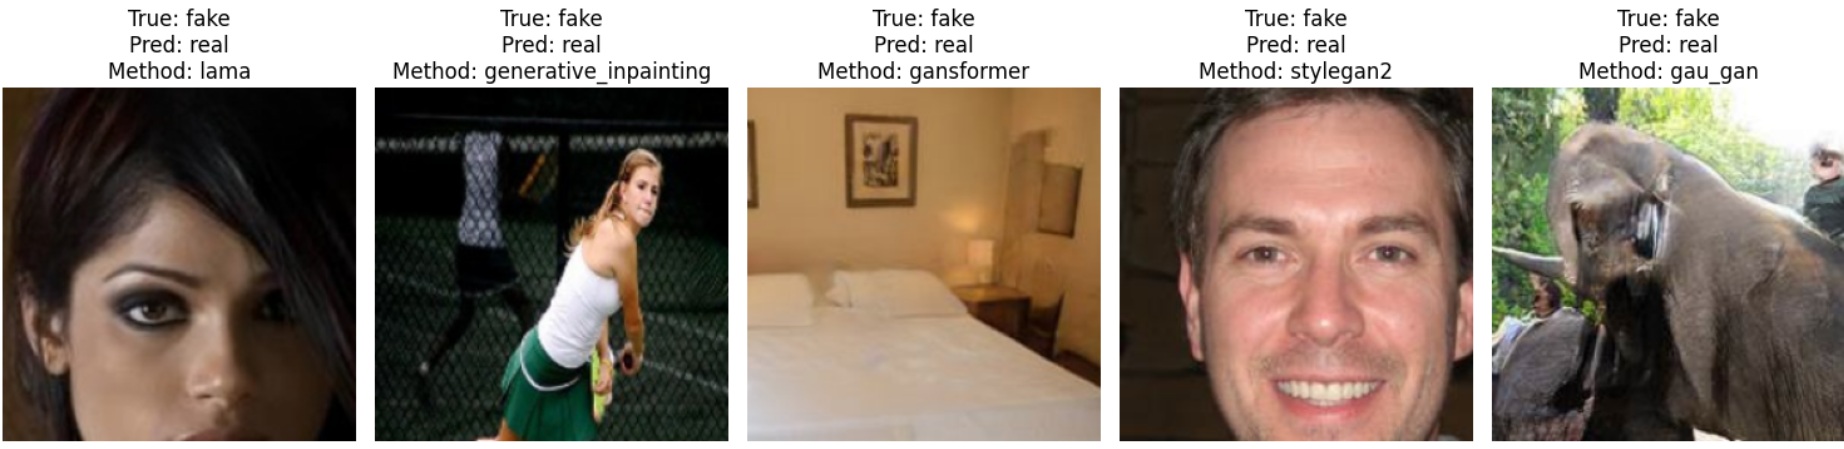
\includegraphics[width=0.76\textwidth]{figs/fake_images.png}
\end{figure}


% \begin{figure}[ht]
%     \centering
%     \begin{minipage}{0.35\textwidth}
%         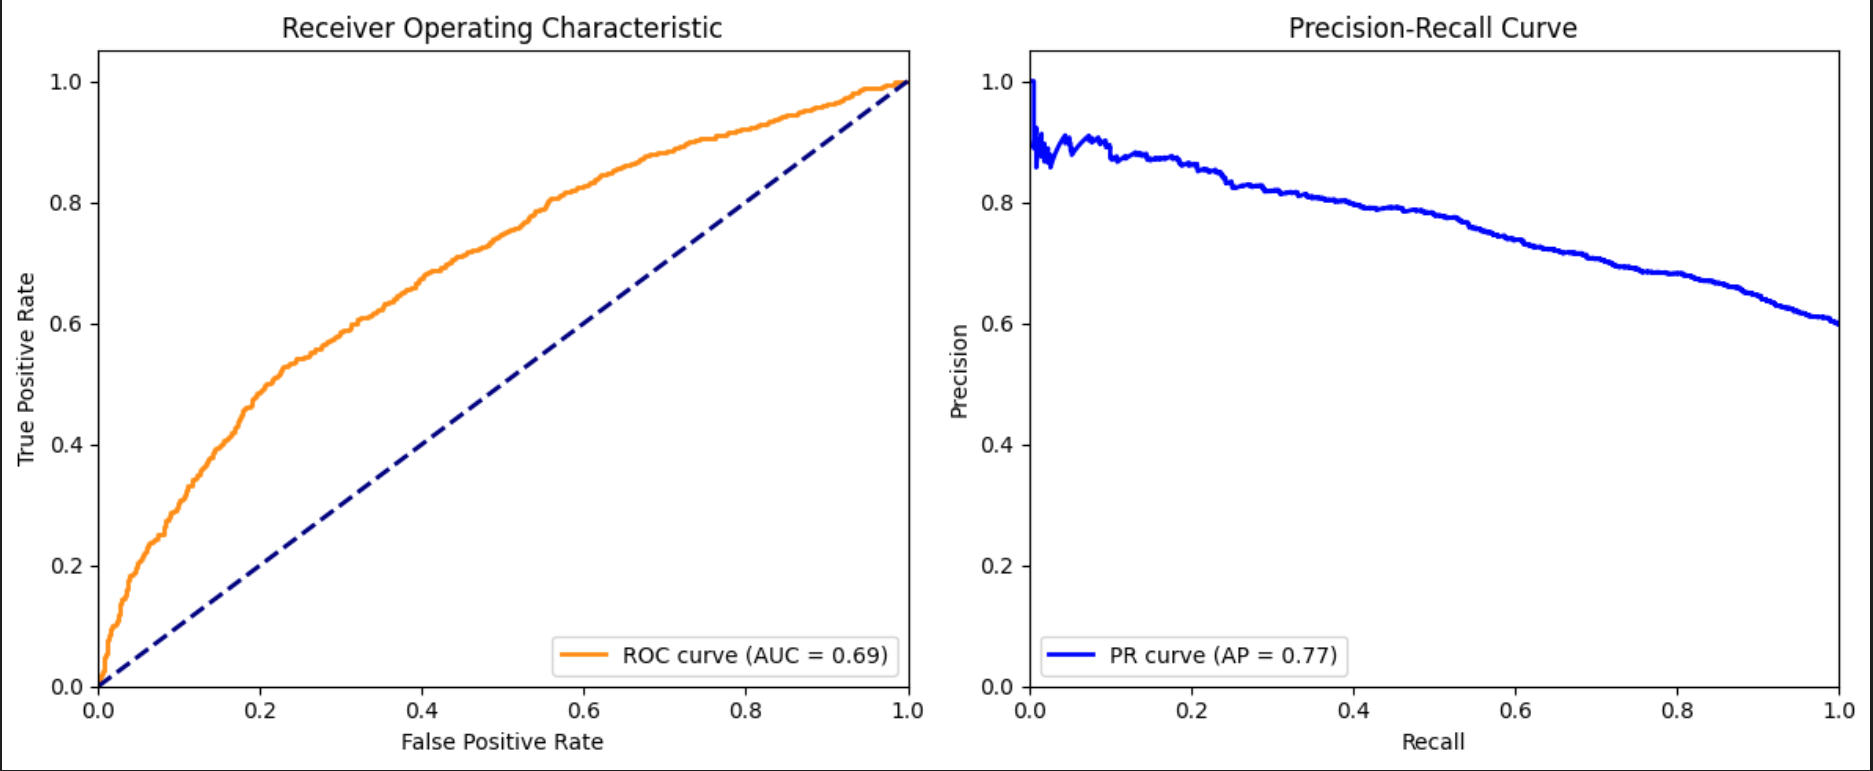
\includegraphics[width=\linewidth]{figs/PR_ROC.png}
%     \end{minipage}
%     \hspace{30pt}
% \end{figure}
\end{frame}
%----------------------------------------------------------------------------------------------------------
\begin{frame}{Clip}
Отображение $\bm{F}: \mathbb{N}_0^{H \times W \times C} \rightarrow \{ 0, 1 \}.$ представляет из себя композицию двух отображений: $\bm{F} = \bm{f} \circ \bm{g}$, где:
\begin{center}
    $\bm{f}: \mathbb{N}_0^{H \times W \times C} \rightarrow \mathbb{R}^{d}$ ~--- векторизация изображения
\end{center}
\begin{center}
    $\bm{g}: \mathbb{R}^{d} \rightarrow \{ 0, 1 \}$ ~--- классификатор
\end{center}
В статье для обучения $\bm{F}$ обучается только голова классифкатора $\bm{g}$, а $\bm{f}$ фиксировано и не обучается. Для векторизатора $\bm{f}$ рассматривается Clip от OpenAI. 
\end{frame}
%----------------------------------------------------------------------------------------------------------

\begin{frame}{Roc-Auc, PR-curve и другие}
\begin{center}
\begin{tabular}{|c|c|c|c|}
\toprule
\hline
accuracy & precision & recall & f1-score \\
\hline
0.689 & 0.679 & 0.655 & 0.658 \\
\hline
\bottomrule
\end{tabular}
\end{center}
\begin{figure}
\centering
\includegraphics[width=0.76\textwidth]{figs/base_Roc_Pr.png}
\end{figure}
\end{frame}
%----------------------------------------------------------------------------------------------------------
\begin{frame}{Увелечение выхода сети}
\begin{figure}
\centering
\includegraphics[width=0.56\textwidth]{figs/3_models_sheme.png}
\end{figure}
\end{frame}
%----------------------------------------------------------------------------------------------------------
\begin{frame}{Графики обучения}
\begin{figure}
\centering
\includegraphics[width=0.76\textwidth]{figs/train_curve.png}
\end{figure}

\begin{figure}
\centering
\includegraphics[width=0.2\textwidth]{figs/3_models_train.png}
\end{figure}

\end{frame}
%----------------------------------------------------------------------------------------------------------
\begin{frame}{Промежуточные результаты}
В работе были проанализированы разные модели и результаты показали, что:
\begin{itemize}
    \item Усложненная модель повысила качество по всем параметрам
    \item Многоклассовая классификация себя не опровдала
\end{itemize}
Ещё планируется сделать:
\begin{itemize}
    \item Разобраться с проблемами многоклассовой классификации и попробовать меньшее число классов
    \item Побобрать конкретные модели для конретных методов и протестировать эту модель
\end{itemize}
\end{frame}
%----------------------------------------------------------------------------------------------------------
\end{document} 
